\chapter{Software design}
\label{ch:software_design}
In this chapter the design of the software and the  external libraries used are briefly described. 

The code has been implemented in the ROS framework (Robot Operating System) \citep{ROS} using \ttt{C++} as programming language. 
The external libraries used are Point Cloud Library (PCL) \citep{PCL}, an open source library which provides a wide array of tools for 3D perception, and the Flexible Collision Library (FCL) \citep{pan2012fcl}, an open source  library for collision detection.

The algorithm is mainly based on the PCL library which is used to do the following operations: filtering, segmentation, plane estimation, principal component analysis, projections onto the table plane and convex hulls.
The FCL library was used only for collision detection between the convex hulls of the objects and the gripper as well. 

The planner used is the Fast Downward planner \citep{helmert2006fast}. To get a plan the binary file of planner is called giving as inputs a domain and a problem description in PDDL syntax.

 
\iffalse
For the collision checking the Flexible Collision Library (FCL) \citep{pan2012fcl} has been used. This library allows to define the collision problem in a simpler manner than other more famous collision libraries such as \textit{Bullet} \citep{Bullet}, and it can work with different objects shapes such as box, spheres, cone, convex, mesh and octree. 
The main library used in this work is the Point Cloud Library (PCL) \citep{PCL_}, which allows some methods to create an object shape from a point cloud.

\begin{enumerate}
\item Nodes
\item Ros graph 
\item simulation
\item PCL - FCL 
\end{enumerate}
\fi

\paragraph{ROS}
The algorithm has been developed by using different nodes in order to have a modular code. 
The nodes implemented are:
\begin{itemize}
\item a node to segment the objects and estimating the table plane coefficients,
\item a node to generate the states having as input the segmented objects and the table plane,
\item a node that, given the states, writes the problem in PDDL syntax, calls the Fast Downward binary file and returns a plan,
\item a node to evaluate the execute the first action of the plan,
\item a decision maker node which controls all the processes and decides the next task to do.  
\end{itemize}
These nodes are implemented as services, that is they receive an input and return an output.
The software architecture is sketched in Figure \ref{fig:architecture}. 
Once the decision maker receives a point cloud from the Kinect it calls the \ttt{segmentation.srv} service giving as input the point cloud and it receives as results the segmented tabletop objects and the plane coefficients. Then it calls the \ttt{states.srv} service giving as input the tabletop objects point clouds and the plane coefficients and it gets as output all the states, as well the poses for the pushing and grasping actions. Then it sends the states to the task planner by requesting the \ttt{plan.srv} service and a plan is obtained. Finally it executes the first plan's action calling the \ttt{execute.srv} service. The result of this service is a boolean variable which specifies if the requested action has the inverse kinematic feasible. If it is not feasible, the decision maker adds to the states the \ttt{ik\_unfeasible} state for that action and recalls the \ttt{plan.srv} service until a feasible plan is returned or there exist no plans.
Once the action has been executed it waits to receive a point cloud from the Kinect and all the process is repeated until no objects stand on the table. If no plans exist could be fault of the segmentation, therefore if there are objects on the table the algorithm is iterated until the robot can do something.
\begin{figure}[h]
\centering
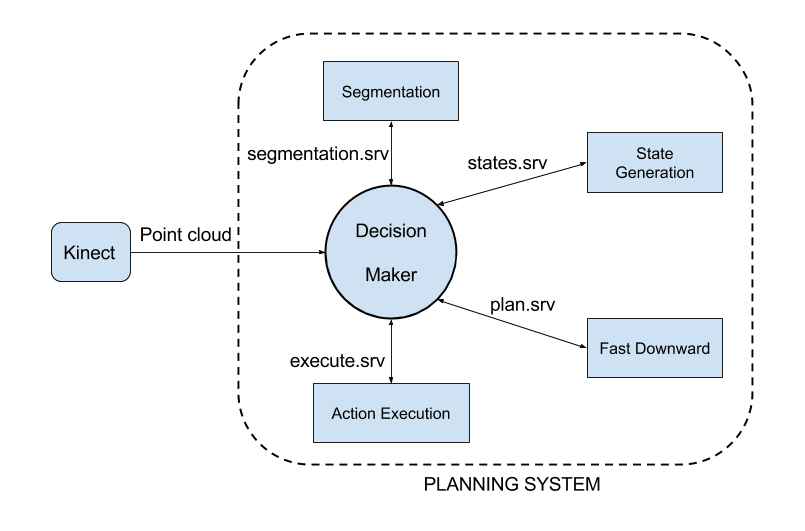
\includegraphics[width=14cm]{Img/software/Software_arquitecture.png}
\caption{Software architecture.}\label{fig:architecture}
\end{figure}


\paragraph{Simulation}
Before to test the implemented algorithm with the real robot it was first tested in simulation with Gazebo\citep{koenig2004design}. A simple URDF model of the gripper (with no joints) was designed in order to simulate the pushing action. Unfortunately, the modelling of the gripper was restricted only to reproduce the closed gripper model (the modelled gripper cannot open and grasp). For this reason in the simulation the objects are always supposed to be grasped successfully, for this aim they are removed manually by the user when the robot executes the grasping action. To validate the correctness of the action to execute the RVIZ package\citep{RVIZ} has been used.  

In the simulation the real set up is accurately reproduced (Figure \ref{fig:sim_setup}). A simulation of the planning system is depicted in Figure \ref{fig:simulation} for a simple problem.
The first plan returned is: \ttt{(push\_dir1 o2) (push\_dir1 o0) (grasp o2) (grasp o1) (grasp o0)}. While the real executed plan is: \ttt{(push\_dir1 o2) (grasp o2) (push\_dir1 o0) (grasp o1) (grasp o0)}. The difference is only that it swaps the second action with the third one, this because the two plans have the same length and at every new frame the system replans again considering it as a problem uncorrelated to the previous one. For the same reason, as long the plan is executed the labels of the objects could change at every new frame. %In this example is possible appreciating that the replanning is useless, asserting the quality of the first computed plan. 

% (it is possible seeing the video of the simulation in ...).

After the algorithm was asserted to work as expected in simulation we moved to perform experiments with real robot. 

\begin{figure}
\centering
\begin{subfigure}[h]{0.45\textwidth}
\centering
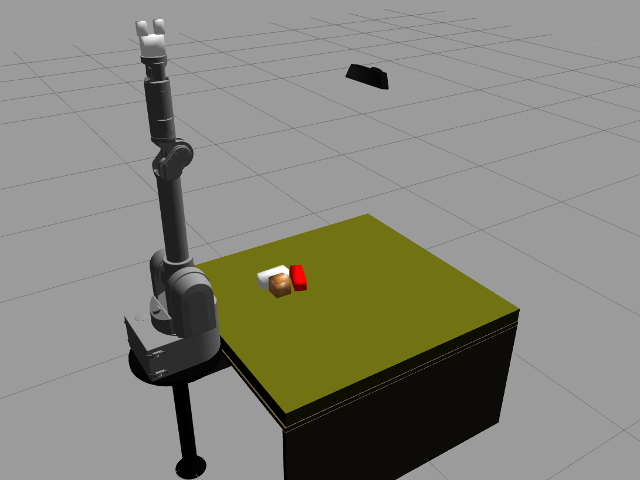
\includegraphics[width=6cm]{Img/simulation/setup_sim.png}
\caption{Simulation of the real set up}\label{fig:sim_setup}
\end{subfigure}
\begin{subfigure}[h]{0.45\textwidth}
\centering
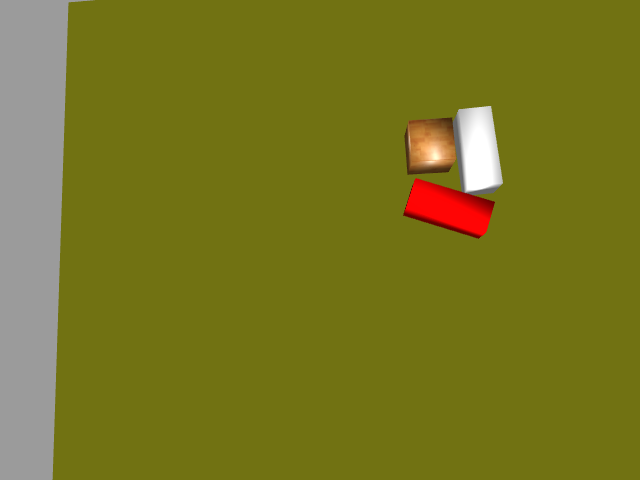
\includegraphics[width=6cm]{Img/simulation/image.png}
\caption{Kinect's view}
\label{fig:sim_kinect}
\end{subfigure}
\begin{subfigure}[h]{0.45\textwidth}
\centering
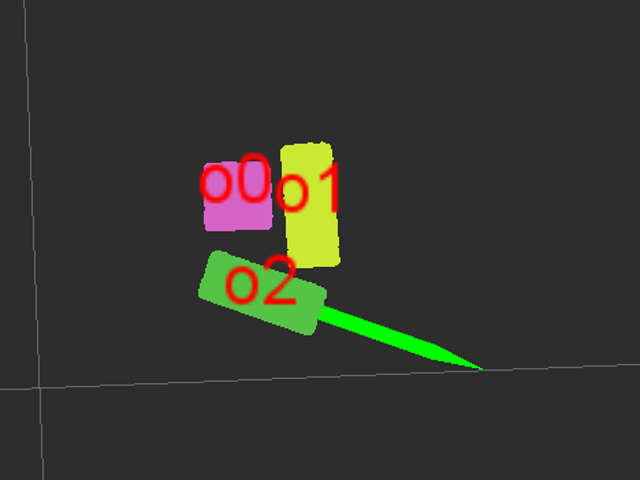
\includegraphics[width=6cm]{Img/simulation/action1.png}
\caption{Visualization in RVIZ of the objects and the action to execute (\ttt{(push\_dir1 o2)}).}
\label{fig:sim_rviz}
\end{subfigure}
\begin{subfigure}[h]{0.45\textwidth}
\centering
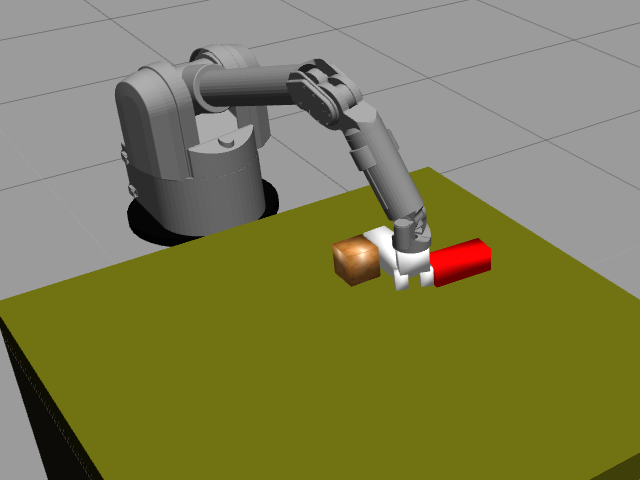
\includegraphics[width=6cm]{Img/simulation/pushing.png}
\caption{Execution of the first plan's action (\ttt{(push\_dir1 o2)}).}\label{fig:sim_push}
\end{subfigure}
\begin{subfigure}[h]{0.45\textwidth}
\centering
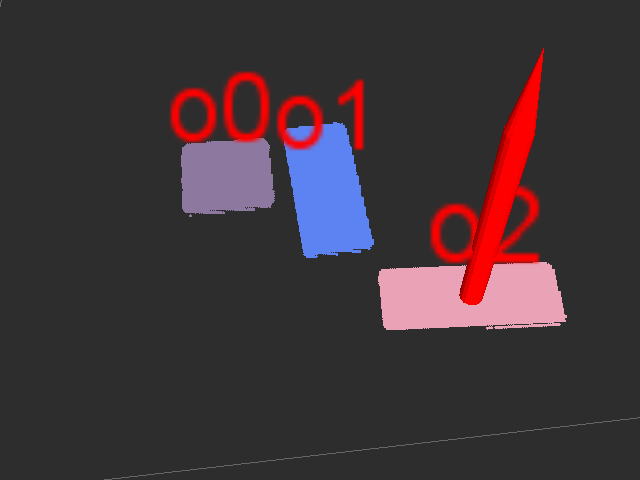
\includegraphics[width=6cm]{Img/simulation/action2.png}
\caption{Visualization in RVIZ of the objects and the action to execute (\ttt{(grasp o2)}).}\label{fig:action2}
\end{subfigure}
\begin{subfigure}[h]{0.45\textwidth}
\centering
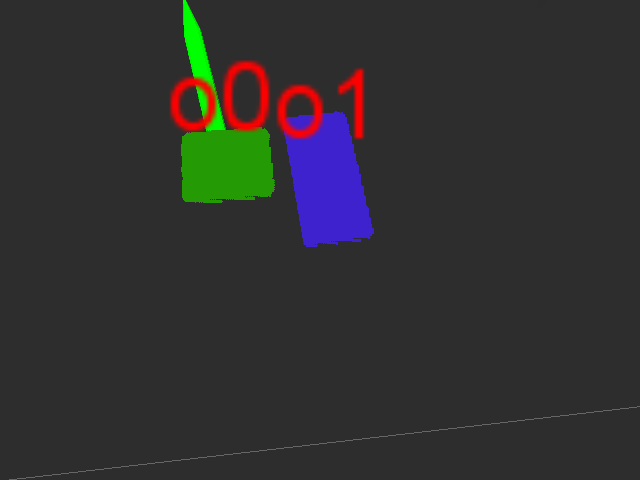
\includegraphics[width=6cm]{Img/simulation/action3.png}
\caption{Visualization in RVIZ of the objects and the action to execute (\ttt{(push\_dir1 o0)}).}\label{fig:action3}
\end{subfigure}
\caption{Simulation in Gazebo of a simple experiment.}\label{fig:simulation}
\end{figure}